\documentclass{article}

\usepackage{tikz}
\usepackage{pdfpages}
\usepackage{parskip}
\usepackage{amsmath}
\usepackage[margin=.6in]{geometry}

\begin{document}
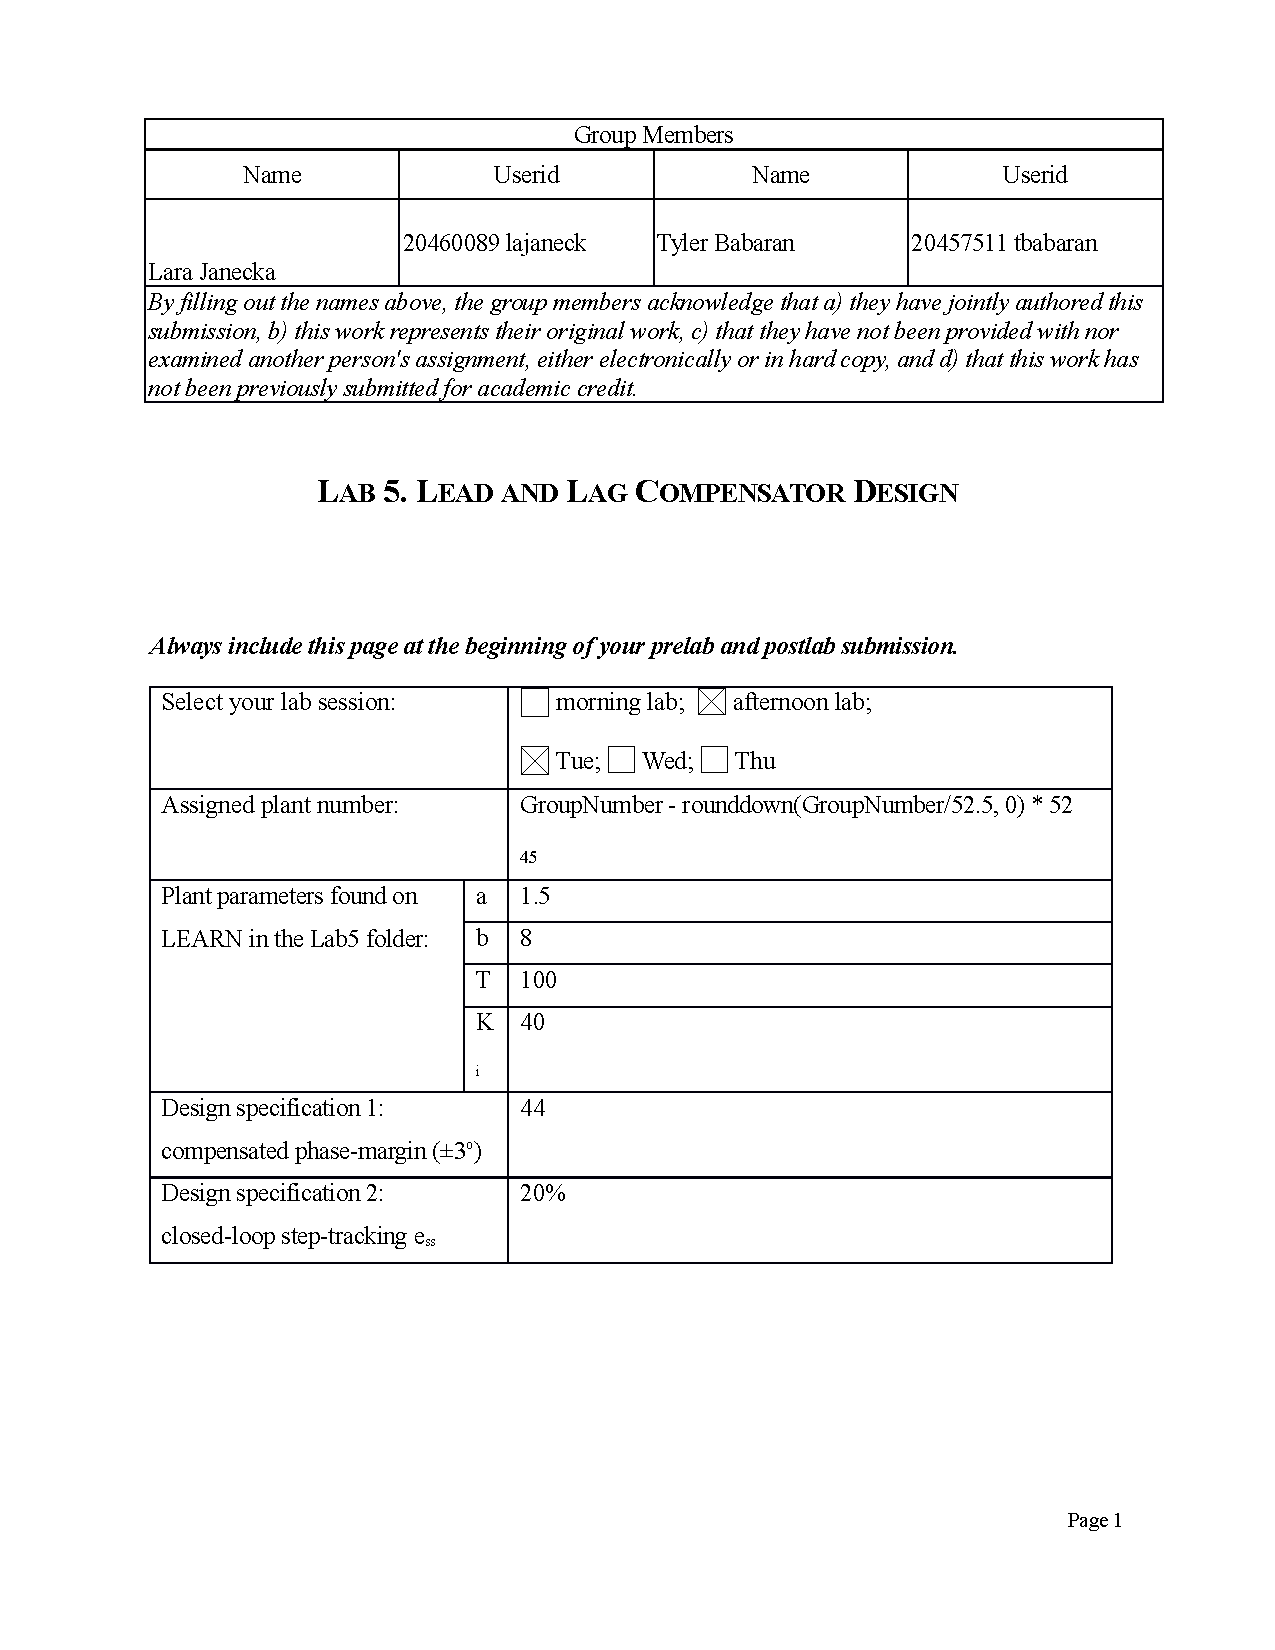
\includepdf[pages={1}]{page1.pdf}
\section{Question 1} % (fold)
\label{sec:question_1}
\subsection{a: transfer function} % (fold)
\label{sub:a_}
\begin{align*}
\text{P(S)} &= \frac{K_ibT}{s(s+aT) + K_ibT}\\
\text{P(S)} &= \frac{40 * 8 * 100}{s(s+1.5*100) + 40 * 8 * 100}\\
\text{P(S)} &= \frac{32000}{s^2 + 150s + 32000}\\
\end{align*}
% subsection a_ (end)

\subsection{b: natural frequency and dampening ratio} % (fold)
\label{sub:b_}
\begin{align*}
\omega_n &= \sqrt{K_ibT}\\
    &= \sqrt{32000}\\
    &= 178.89\\
\zeta &= \frac{aT}{2\omega_n}\\
    &= \frac{150}{2*178.89}\\
    &= 0.42\\
\end{align*}
% subsection b_ (end)

\subsection{c: time to first peak} % (fold)
\label{sub:c_time_to_first_peak}
\begin{align*}
T_p &= \frac{\pi}{\omega_n\sqrt{1-\zeta^2}}\\
T_p &= \frac{\pi}{178.89\sqrt{1-0.42^2}}\\
T_p &= 0.019s\\
\end{align*}
% subsection c_time_to_first_peak (end)

\subsection{d: overshoot} % (fold)
\label{sub:d_overshoot}
\begin{align*}
OS &= 100e^{\frac{-\zeta\pi}{\sqrt{1-\zeta^2}}}\\
    &= 100e^{\frac{-0.42\pi}{\sqrt{1-0.42^2}}}\\
    &= 23\%
\end{align*}
% subsection d_overshoot (end)

\subsection{e: low frequency gain} % (fold)
\label{sub:e_low_frequency_gain}
\begin{align*}
\text{low frequency gain} &= 20\log P(j\omega)\\
    &= 20\log (\frac{32000}{(0.01)^2 + 150j(0.01) + 32000})\\
    &= 20\log (\frac{32000}{32000})\\
    &= 20\log 1\\
    &= 0\\
\end{align*}

% subsection e_low_frequency_gain (end)

% section question_1 (end)
\section{Question 2} % (fold)
\label{sec:question_2}
Since the plant is a system of type zero:
\begin{align*}
K_p &= lim_{s \to 0} KP(S)\\
    &= lim_{s \to 0} K\times \frac{32000}{s^2 + 150s + 32000}\\
    &= K\\
e_{ss} &= \frac{1}{1+K_p}\\
        &< 0.2\\
        &\implies K > 4
\end{align*}

% section question_2 (end)

\section{Question 3} % (fold)
\label{sec:question_3}
\begin{figure}[!htbp]
    \centering
    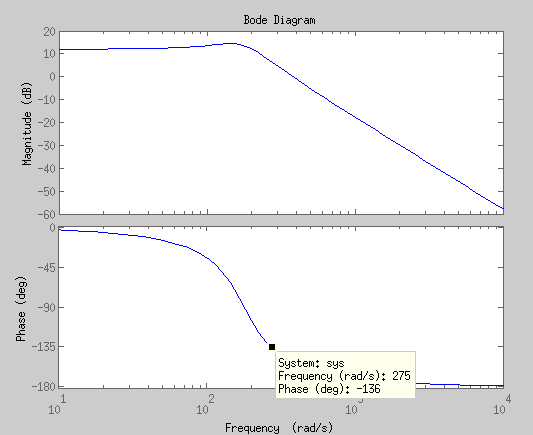
\includegraphics[width=0.95\textwidth]{prop_sys2.png}
    \caption{Bode Plot of $KP(S)$}
\end{figure}
We need to a gain cross over frequency of 275 rad/s. The gain at this frequency is 6.62

The gain at the desired cross over frequency must be changed to be 0.
\begin{align*}
    20\log \alpha &= -6.62\\
    \alpha &= 0.467
\end{align*}

The phase needs to stay the same at the new cross over frequency.
\begin{align*}
\frac{10}{\alpha \tau} &= 275\\
\frac{10}{0.467 \tau} &= 275\\
\tau &= 0.078
\end{align*}

Plug these values into C(S)
\begin{align*}
\text{C(S)} &= K\frac{\alpha\tau s + 1}{\tau s + 1}\\
    &= 4\frac{0.467 * 0.078 s + 1}{0.078 s + 1}\\
    &= 4\frac{0.036 s + 1}{0.078 s + 1}\\
\end{align*}

From the transfer function of C(S) we can calculate the location of our zero and pole
\begin{align*}
0.036 z_{lead} + 1 &= 0\\
z_{lead} &= -27.48\\
0.078p_{lead} + 1 &= 0\\
p_{lead} &= -12.82\\
\end{align*}
% section question_3 (end)

\section{Question 4} % (fold)
\label{sec:question_4}

\begin{figure}[!htbp]
    \centering
    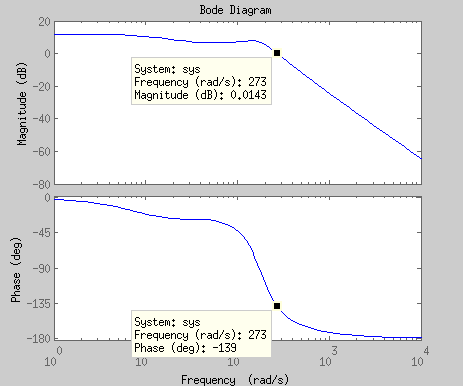
\includegraphics[width=0.95\textwidth]{sim_lag_rad.png}
    \caption{Frequency response of lag compensated system}
\end{figure}

This shows the desired phase margin(or close to it) at the cross over frequency indicating our compensator works.

\begin{figure}[!htbp]
    \centering
    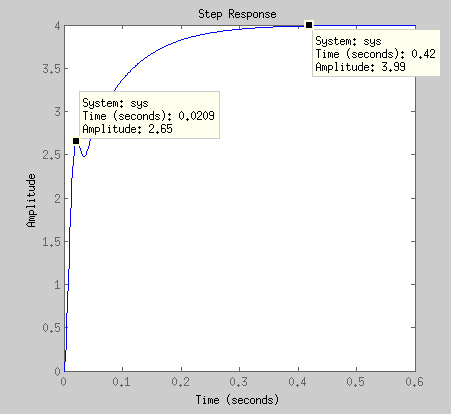
\includegraphics[width=0.95\textwidth]{sim_lag_step.png}
    \caption{Step response of lag compensated system}
\end{figure}

\newpage
% section question_4 (end)





\section{Question 5} % (fold)
\label{sec:question_5}
\begin{figure}[!htbp]
    \centering
    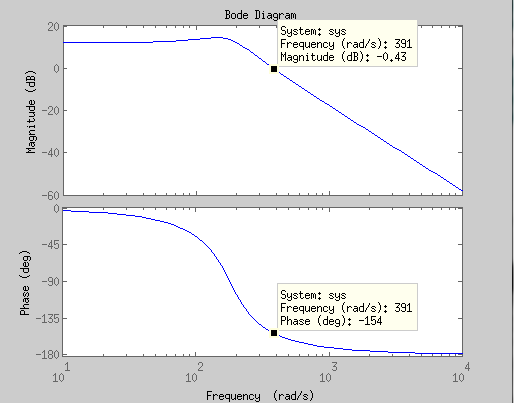
\includegraphics[width=0.95\textwidth]{prop_sys.png}
    \caption{Bode Plot of $KP(S)$}
\end{figure}
The cross over gain frequency: $\omega_{gc} = 390$ rad/s

phase margin: $PM = 25$

We need to add 19 degrees of phase margin, we'll add 24 degrees instead.

Here we calculate for $\alpha$
\begin{align*}
24 &= \sin^{-1}(\frac{\alpha - 1}{\alpha + 1})\\
0.41 &= \frac{\alpha - 1}{\alpha + 1}\\
0.41\alpha + 0.41 &= \alpha - 1\\
\alpha = 2.39
\end{align*}

By setting the $\omega_{max} = \omega_{gc}$ we can calculate $\tau$.
\begin{align*}
\omega_{max} = \frac{1}{\sqrt{\alpha}\tau}\\
390 = \frac{1}{\sqrt{2.39}\tau}\\
\tau &= 0.00166
\end{align*}

We then plug in the known values of $\alpha$ and $\tau$ to get the transfer function of C(S).
\begin{align*}
\text{C(S)} &= K\frac{\alpha\tau s + 1}{\tau s + 1}\\
    &= 4\frac{2.39 * 0.00166 s + 1}{0.00166 s + 1}\\
    &= 4\frac{0.00396 s + 1}{0.00166 s + 1}
\end{align*}

From the transfer function of C(S) we can calculate the location of our zero and pole
\begin{align*}
0.00396z_{lead} + 1 &= 0\\
z_{lead} &= -252.3\\
0.00166p_{lead} + 1 &= 0\\
p_{lead} &= -602.41\\
\end{align*}

% section question_5 (end)
\section{Question 6} % (fold)
\label{sec:question_6}
\begin{figure}[!htbp]
    \centering
    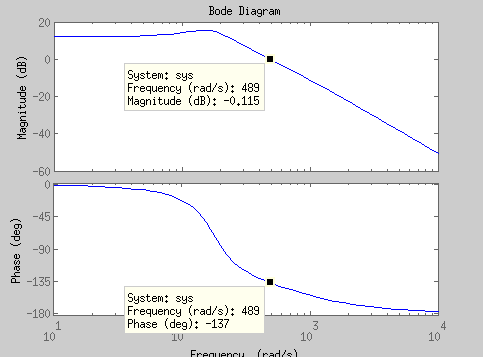
\includegraphics[width=0.95\textwidth]{sim_lead_rad.png}
    \caption{Frequency response of lead compensated system}
\end{figure}
This shows the phase margin of 43 which is very close to the desired phase margin of 44.

\begin{figure}[!htbp]
    \centering
    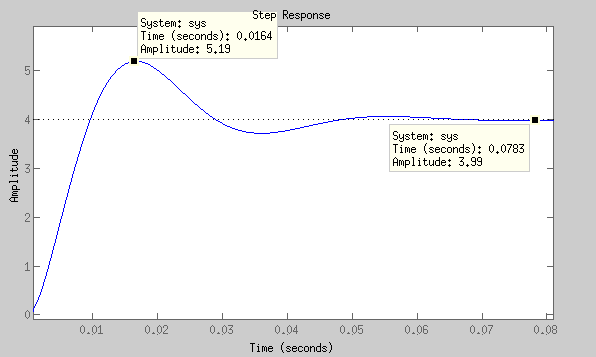
\includegraphics[width=0.95\textwidth]{sim_lead_step.png}
    \caption{Step response of lead compensated system}
\end{figure}

This shows a time to first peak of 0.0164 which is very close to our calculated time to first peak of 0.019. The overshoot on this is roughly 30\% which is also close to our calculated value of 23\%.


\begin{table}[!htbp]
\centering
    \begin{tabular}{|c|c|}
        \hline
        $z_{lead}$ & -252.3 \\
        \hline
        $p_{lead}$ & -602.41 \\
        \hline
        $Gain_{1}$ & 4 \\
        \hline
        $z_{lag}$ & -27.48 \\
        \hline
        $p_{lag}$ & -12.82 \\
        \hline
        $Gain_{2}$ & 4 \\
        \hline
    \end{tabular}
    \caption{Prelab results for the lead and lag compensator}
\end{table}
% section question_6 (end)

\end{document}
